\documentclass[xcolor=dvipsnames, notes]{beamer}
%\documentclass[xcolor=dvipsnames]{beamer}

\usetheme{Warsaw}

\usepackage{amsmath}
\usepackage{amsthm}
\usepackage{graphicx}

\title{Validating Optimizations of Concurrent C/C++ Programs}
\subtitle{Soham Chakraborty and Viktor Vafeiadis}

\author{Presented by \\ Akshay Gopalakrishnan}

\begin{document}

    \begin{frame}

        \maketitle

    \end{frame}

    %Introduction 
    \begin{frame}{Introduction}
        
        \begin{itemize}
            \item Lot of optimizations done at the LLVM IR level for C/C11 programs.
            \item However, very conservative when it comes to transformations involving shared memory accesses.
            \item Prior work formalized a major fragment of the LLVM memory model.
            \item This helped to prove that many transformations not done were infact safe to do.
            \item The current work introduces a validator that verifies whether LLVM transformations are safe to do wrt the C11 and LLVM memory model.
        \end{itemize}
        
    \end{frame}

    \begin{frame}{Simple example}

        \begin{figure}
            \makebox[\textwidth][c]{
                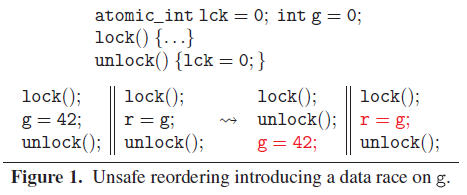
\includegraphics[scale=0.7]{OPT_INVALID.PNG}
            }
        \end{figure}
    \end{frame}

    %C11 and LLVM memory model
    \begin{frame}{C11/LLVM memory model: Common elements}

        Partial orders on program elements
        \begin{itemize}
            \item Program order. 
            \item Syncrhonize with order.
            \item Reads-from. 
        \end{itemize}

        Access orders:
        \begin{itemize}
            \item Non-Atomic - default access mode of shared memory.
            \item Release - for write accesses. 
            \item Acquire - for read accesses. 
            \item Sequentially consistent - default atomic access mode for shared memory.
        \end{itemize}

    \end{frame}

    %Example to show why LLVM and C11 have different concepts of memory model 
    \begin{frame}{C11/LLVM memory model: Example showing their difference}
        
        \begin{figure}
            \makebox[\textwidth][c]{
                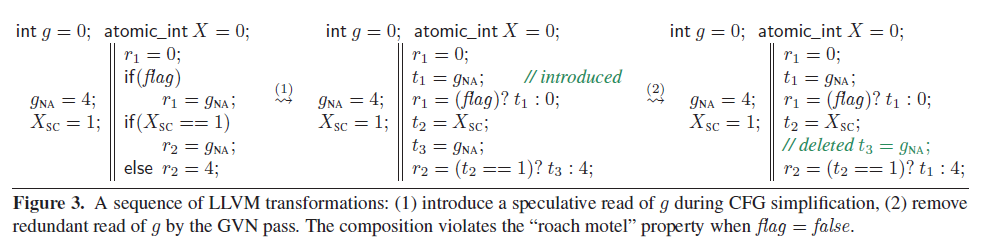
\includegraphics[scale=0.5]{LLVM_OPT_EX1.PNG}
            }
        \end{figure}

    \end{frame}


    \begin{frame}{Explaination}

        \begin{itemize}
            \item The first transformation reorders the read of $g_{NA}$ to be before the conditional.\
            \item This transformation is invalid under C11 memory model, but is extensively done in LLVM.
            \item The reason for this is the second transformation which does Global Value Numbering (a form of redundant code elimination).
            \item These two transformations in unison prevent multiple reads from $g_{NA}$.
            \item While it is safe to perform the second transformation in C11, the first violates the std "roach motel" reordering constraint, thus giving us a new outcome for when flag is set to false.
        \end{itemize}
        

    \end{frame}

    %Summary of other concurrency bugs
    \begin{frame}{Other errors due to transformations}

        \begin{figure}
            \makebox[\textwidth][c]{
                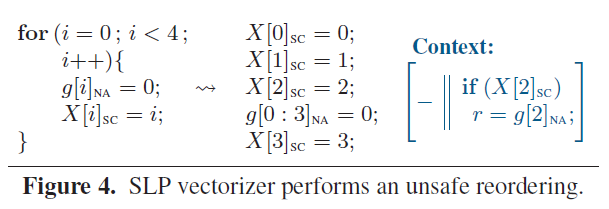
\includegraphics[scale=0.7]{OPT_INVALID_2.PNG}
            }
        \end{figure}

        \begin{figure}
            \makebox[\textwidth][c]{
                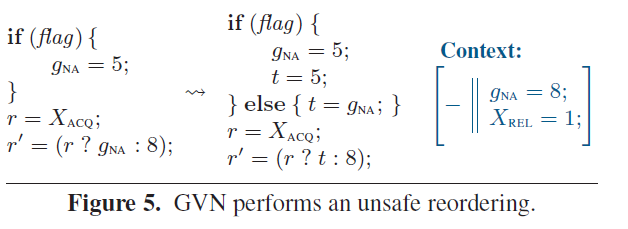
\includegraphics[scale=0.7]{OPT_INVALID_3.PNG}
            }
        \end{figure}

    \end{frame}

    \note{
        Both these examples exhibit unsafe reordering. 
        It is interesting to note that several complex transformations involve this basic transformation at its elementary level.
    }

    %Validation approach summary
    \begin{frame}{Validation Approaches}

        Two kinds:
        \begin{itemize}
            \item Compiler independent matching - No IR or Language specific constructs required (only memory model suffices).
            \item LLVM specific matching - Makes use of IR metadata to improvise validation.
        \end{itemize}
        
        Three possible results of matching:
        \begin{itemize}
            \item Correct - transformation is safe and valid. 
            \item Possible error - transformation is unsafe (one of them).
            \item Unknown - cannot decisively conclude on the validity (due to loops).
        \end{itemize}
        
    \end{frame}

    \begin{frame}{Compiler Independent Mathcing (CIM)}

        \begin{itemize}
            \item Consider a source program and a target program after performing a set of transformations.
            \item Mark the events in the source and target program using some tags (next slide).
            \item Perform matching between events of source and that of target.
            \item Matchings misaligned (cross matchings) imply reordering applied.
            \item No matching for target event implies Introduction or speculative transformation applied.
            \item No matching for source event implies elimination transformation applied.
            \item Analyze based on this information. 
        \end{itemize}

    \end{frame}

    \begin{frame}{CIM: Basic Tags}

        \begin{itemize}
            \item Non-deletable - Cannot be eliminated.
            \item Conditionally deletable - Can be eliminated subject to another transformation being applied to another event in the same thread.
            \item Immediately Deletable - Can be eliminated right away.
        \end{itemize}
        
    \end{frame}

    \note{
        The conditionally deletable is the most tricky part. It relies on some other transformation to have been done in the source, which is something in my eyes very difficult to assert. Firstly, which transformation and secondly on which events.
        The lack of any proofs given based on their assignment of tagging makes it a little more difficult to have intuition on this tag been given to events.
        They have covered some cases on when to conditionally match, but is it sound ? Also, is it complete?
        Also, note that these tags do not help us decide reordering or Introduction in any way.
    }

    \begin{frame}{CIM: Example using tags}

        \begin{figure}
            \makebox[\textwidth][c]{
                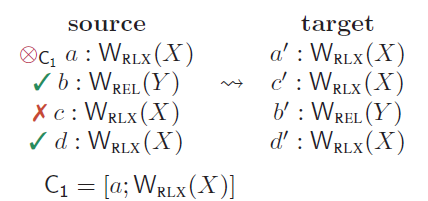
\includegraphics[scale=0.7]{CIM_MATCHING_EX.PNG}
            }
        \end{figure}

    \end{frame}

    \note{

        Note here that the release write to $Y$ is non-deletable (as deleting it would result in syncrhonization errors).
        Additionally, the last write to $X$ is non-deletable (elminiation would result in unsafe behaviors such as reading a previous write not supposed to be visible.)
        The third write is deletable because a write proceeding it replaces its value (also it is relaxed order and a proof for soundness of such a transformation exists). 
        The first one is conditional on the third write being reordered before the release write (as shown in right hand side of figure).
        Note that tagging of conditionally deletable is non-trivial.
    }

    \begin{frame}{CIM: How to mark accesses using tags? }

        Initially, we mark all actions non-deletable and then go on to re-mark them as deletable or conditionally deletable.
        The latter tag is non-trivial to assign, here are a few observations on them:
        \begin{itemize}
            \item Insufficiency of release-acquire pairs: Not sufficient to ensure an event is non-deletable
            \item C11 release sequences: Certain release accesses can also be deleted (if strengthening transformation is performed)
            \item Synchronization access deletion: Although allowed under certain circumstances (low level Fence eliminations), it is avoided at all costs (goes against programmer intention and may cause deadlock).  
        \end{itemize}

    \end{frame}

    \note{
        The release-acquire pair Insufficiency is validated by an example that reorders a release with a subsequent acquire.
        I remember in our analysis for JavaScript, we deemed such a reordering to be invalid as it introduces happens-before cycles.
        More importantly, our reasoning was that this would go against programmer intuition as the synchronizations placed by them should ideally work, and must not suddenly stop due to some addition of syncrhonization by the compiler.
        However, this actually means that a new behavior can be formed. This still has to be proved.
    }

    \begin{frame}{CIM: Matching source with target}

        Once all the marking of events are done, matching follows. Here are the steps taken:
        \begin{itemize}
            \item Match all Synchronization events first. If a mismatch is found, return "Possible Error".
            \item Now for each non-deletable source action not matched, define a window between events that this event cannot be reordered out of. Now match these corner events with target. This window will be our place to search for a match. If a match is not found, it certainly implies an incorrect reordering has been done. Thus we can return Possible Error.
            \item Now for all deletable target actions, we perform the same matching as that of the previous. If a match is not found, we consider it as introduction transformation and analyze further.  
        \end{itemize}

    \end{frame}

    \begin{frame}{CIM: Matching Source with Target cnt'd}

        Any unmatched target action implies introduction transformation. 
        \begin{itemize}
            \item Write/Updates: Atomic is disallowed (Possible Error) but certain cases of non-atomic allowed (Correct).
            \item Reads: Incorrect as per C11 but safe as per LLVM model (Unknown).
            \item Fences: Just adds synchronization so safe (Correct).  
        \end{itemize}

    \end{frame}

    \note{
        Fence introduction, as per my work on JavaScript may be incorrect as if we prove transformations by preserving existing happens-before relations, then this would introduce a cycle.
        This cycle would be illegal. Though one may not observe this cycle in practice.
        This is something to note/observe in our future endeavors tackling transformations.
    }

    \begin{frame}{CIM: Example Matching}

        \begin{figure}
            \makebox[\textwidth][c]{
                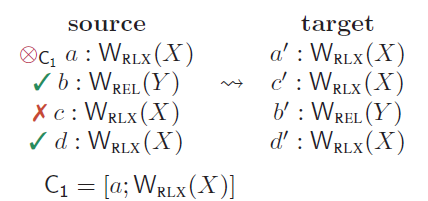
\includegraphics[scale=0.7]{CIM_MATCHING_EX.PNG}
            }
        \end{figure}

        Note: $W_{REL}(X)$ should be non-deletable.

    \end{frame}

    \note{
        The numbers in the matching lines indicate the step number as per previous slide.
    }

    \begin{frame}{CIM: Moving towards Conditional Branching}

        \begin{itemize}
            \item For each target code path, identify a set of source paths.
            \item Apply matching analysis as above for each such pair.
            \item The target program is safe if all such possible mappings are Correct. 
        \end{itemize}
    
    \end{frame}
    %LLVM Specific matching 
    \begin{frame}{LLVM Specific Matching using MetaData (MD)}
       
        \begin{itemize}
            \item LLVM has a feature of attaching metadata to programs that is preserved throughout the pipeline of transformations.
            \item This feature is used to attach information about events and relations to any future events.
            \item This information is used to decide whether transformations performed were safe overall.
            \item Examples of such information added are: OrderedPairs(a,b), PathConditions(a), etc.
        \end{itemize}
        
    \end{frame}

    \begin{frame}{Observations on Testing both Methods: CIM vs MD}

        \begin{itemize}
            \item CIM and MD are extremely accurate (hence the Bugs they found).
            \item CIM misses some errors due to mismatching events and taking some events to be introduced and some eliminated.
            \item MD finds more errors than CIM.
            \item MD has false positives - Due to end-to-end validation error (only see source target, but no intermediate steps).
            \item CIM is better for end-to-end validation.
            \item MD is better for individual step-wise validation.
        \end{itemize}
    \end{frame}

    \note{
        LLVM keeps playing with metadata, sometimes even discards some. 
        This might also be the reason for MD to be having False Positives.
        However, the example the authors used to show MD has false positives seems to show that CIM will also give the same outcome.
        But, this is not the case because the event in target is A, for whcih the only path we get from source is the conditional fails.
        This tells me that they do not particularly work at the value level. 
        This might become problematic as I am unsure how they tackle it. 
    }

    \begin{frame}{Thank you}

        Questions?
    \end{frame}

\end{document}